\section{Avvenimenti di trama}
\begin{figure}[h]
  \centering
  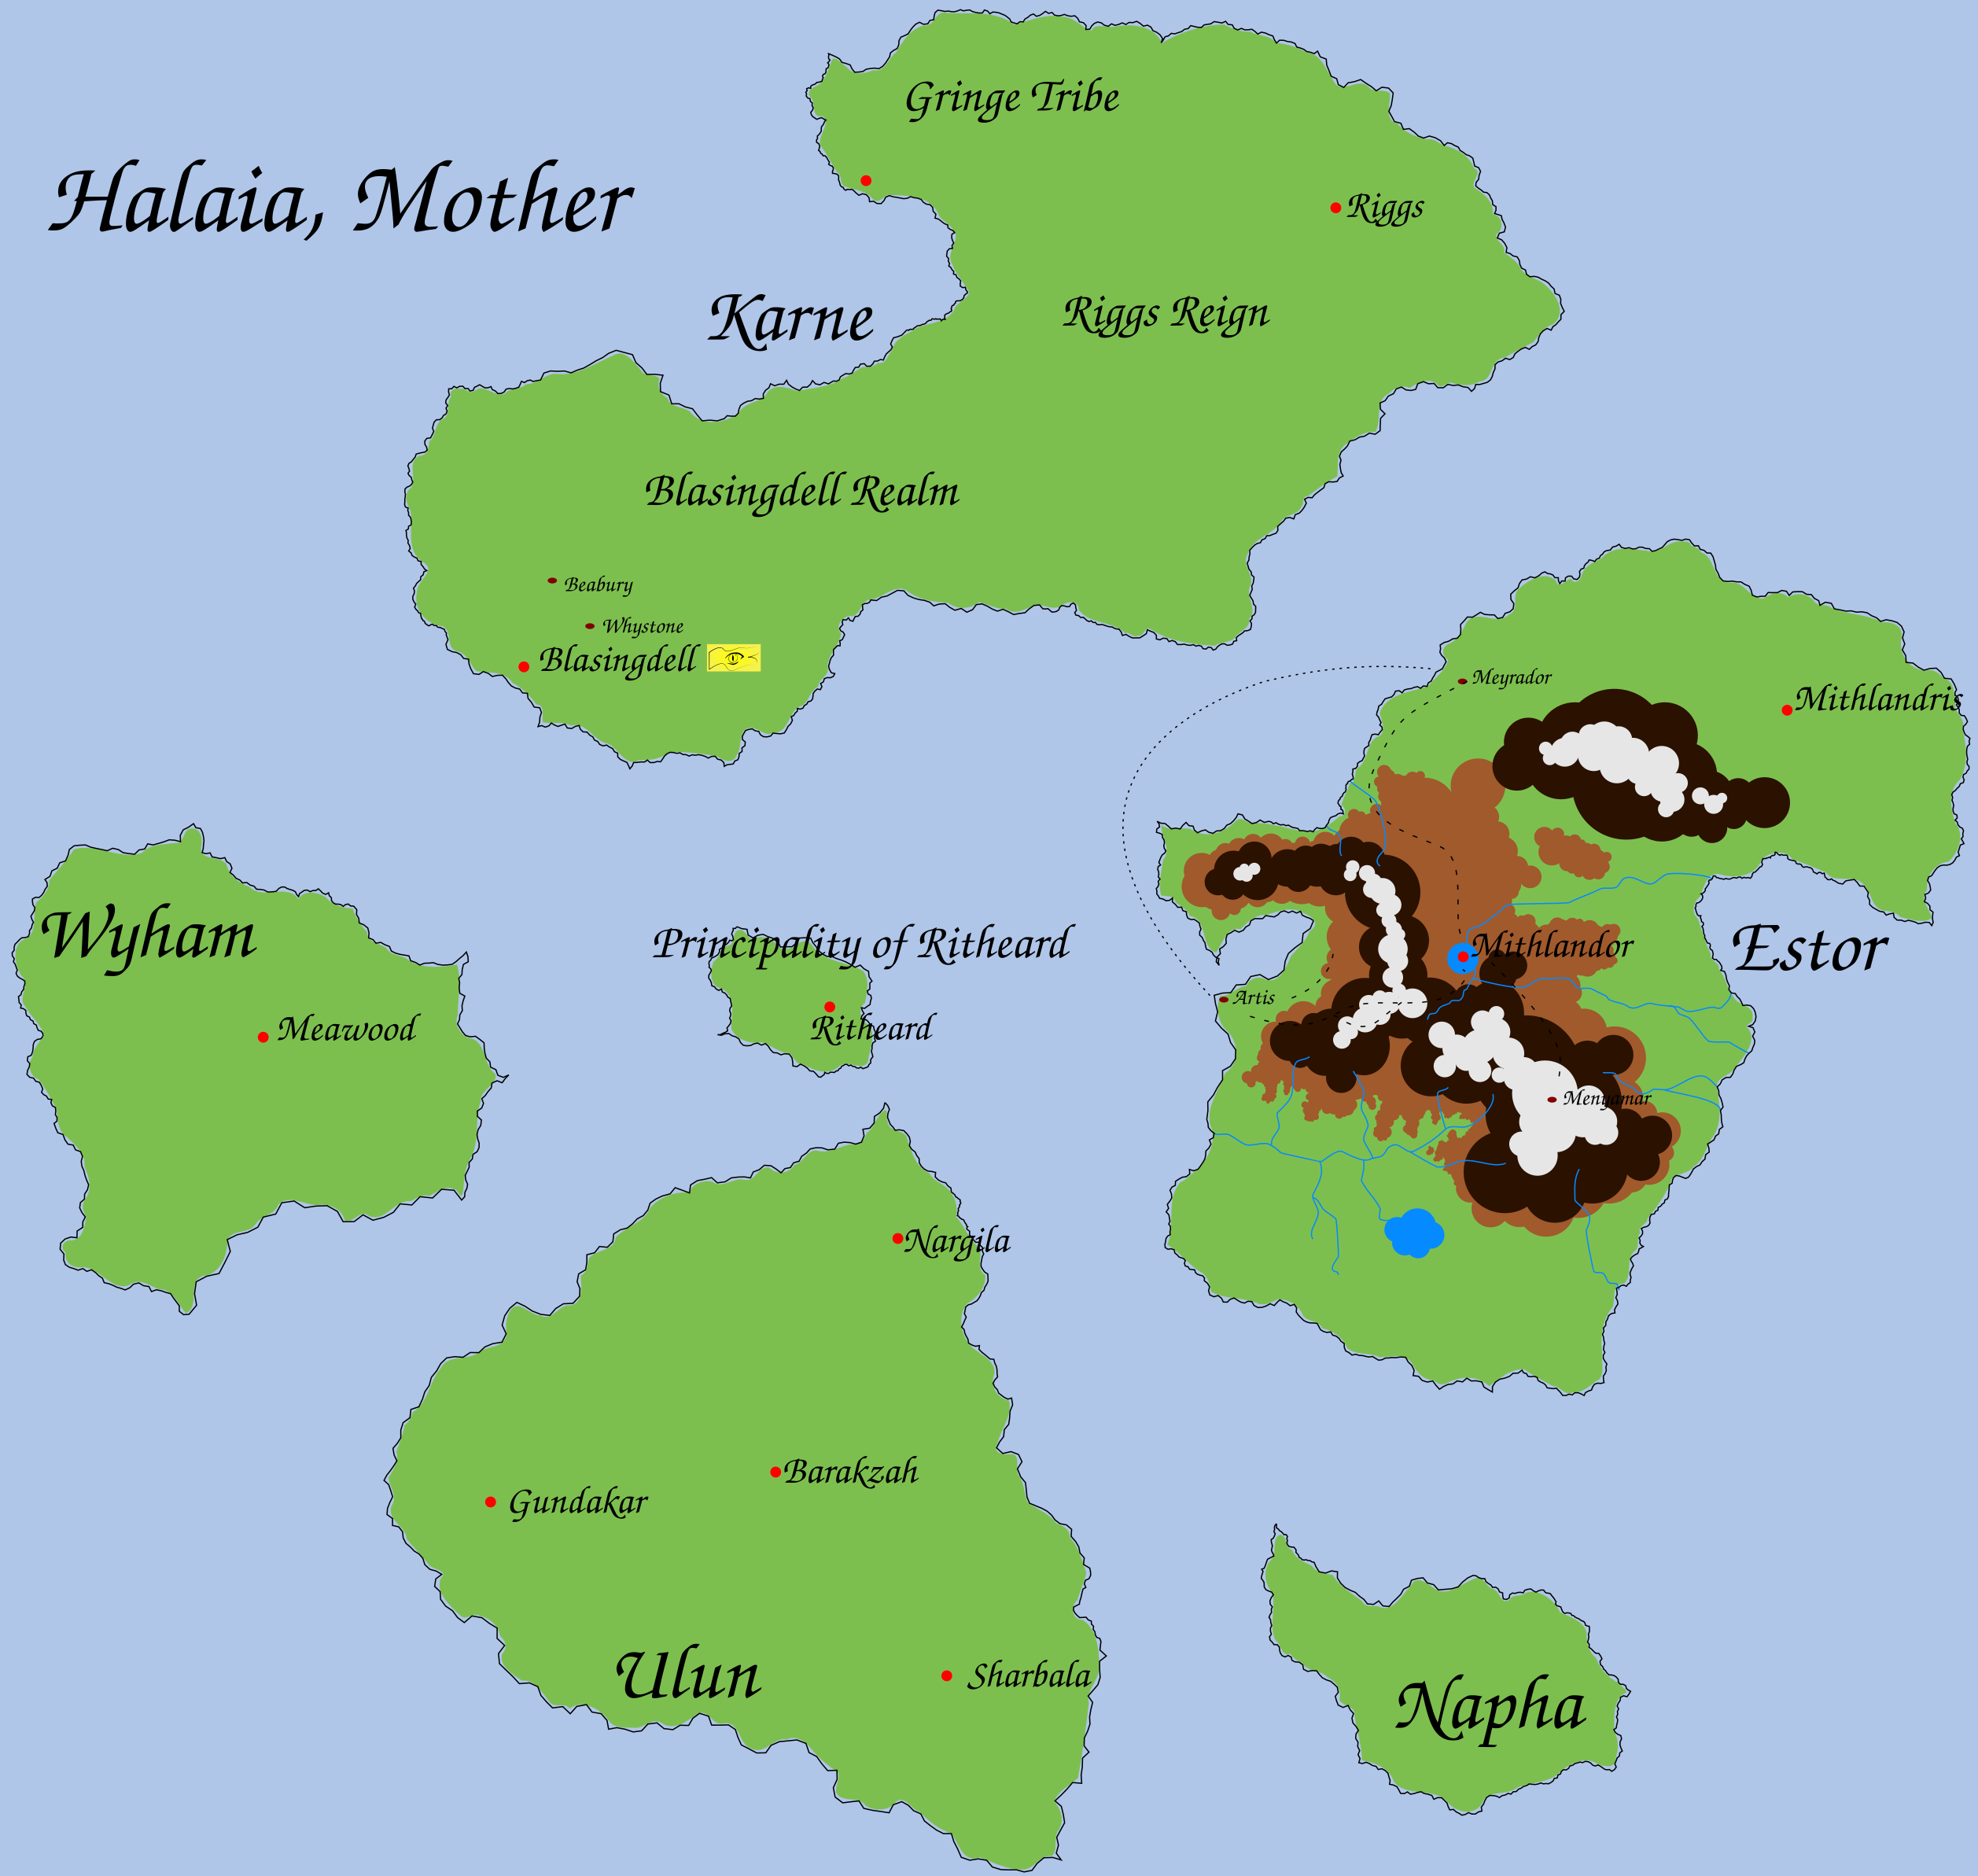
\includegraphics[width=0.5\textwidth]{../../drawings/WorldMap/rect181.png}
  \caption{Mappa del Mondo}
  \label{fig:worldmap}
\end{figure}
\subsection{Guerra tra i regni}
Ombre del Sole sono interessate a compiere un colpo di stato per rovesciare il regno degli umani e
poi degli elfi e prendere il potere.

\begin{commentbox}{Attentato}
  Per mano di Kaligtibur si \`e compiuto un attentato alla vita dei consiglieri della
  famiglia reale regnante a Mithlandor. La colpa non \`e stata ancora data, ci sono
  indagini in corso in citt\`a e i controlli sono molto elevati. Sebbene non sia di
  mentalit\`a razzista, questo avvenimento ha contribuito non poco ad alzare
  i sospetti contro i non elfi.
\end{commentbox}
\begin{commentbox}{Miniera}
  La miniera pare che nasconda dentro di se il cuore di Kraul: un antico artefatto che
  pare permetta di controllare i draghi. Il cuore di Kraul \`e in realt\`a un nome
  locale che si riferisce ad un artefatto molto pi\`u generale chiamato Anima del
  Fuoco che ha origine da grandi fonti di fiamme e calore. Pare che dia il potere di
  controllo del fuoco e chiss\`a quali altri poteri. C'\`e chi dice che dia
  il potere di controllare un drago rosso.
\end{commentbox}